\documentclass[letterpaper, reqno,11pt]{article}
\usepackage[margin=1.0in]{geometry}
\usepackage{color,latexsym,amsmath,amssymb,graphicx, float}
\usepackage{hyperref}

\hypersetup{
colorlinks=true,
linkcolor=magenta,
filecolor=magenta,
urlcolor=cyan,
}

\graphicspath{ {images/} }

\begin{document}
\pagenumbering{arabic}
\title{ELEC 481 Homework 6}
\date{09/06/22}
\author{Xander Naumenko}
\maketitle

{\noindent\bf Question 1a.} 

\[
i^{30}=\frac{130000}{70000}\implies i=2.1\%
.\]

{\noindent\bf Question 1b.} 

\[
    (1+i)^{30}=\left( 1+i'+f+i'f \right)^{30}=\frac{130000}{70000}\implies i'=-0.1\%
.\]

{\noindent\bf Question 1c.} 

\[
F=P \cdot (1+f)^{30}=\$134470
.\]

{\noindent\bf Question 2.} The present value of the costs can be seen in figure \ref{fig:q2} (their NPW is the negative of the SUM result at the bottom). As can be seen the Duro option has a lower cost so should be chosen. 

\begin{figure}[htpb]
    \centering
    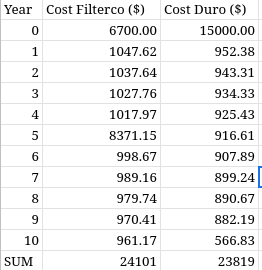
\includegraphics[width=0.8\textwidth]{q2}
    \caption{NPW of the costs for the two options for question 2. }
    \label{fig:q2}
\end{figure}

{\noindent\bf Question 3a.} See the revenue stream in figure \ref{fig:q3}. Using the excel IRR function we find the monthly interest rate is 2.73\%. This corresponds to an annual interest rate of $1.0273^{12}-1=38.2\%$. 

\begin{figure}[htpb]
    \centering
    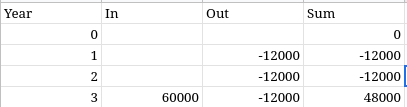
\includegraphics[width=0.8\textwidth]{q3}
    \caption{Revenue stream for question 3}
    \label{fig:q3}
\end{figure}

{\noindent\bf Question 3b.} Adjusting this rate we get: 
\[
i'=\frac{i-f}{1+f}=31.3\%
.\]

{\noindent\bf Question 4a.} 

\[
F=10000\cdot 1.044^{15}=\$19077
.\]

{\noindent\bf Question 4b.} Five years away value: 

\[
F=10000\cdot (\frac{0.044-0.052}{1.052}+1)^5=\$9626
.\]

After 10 years: 
\[
F=9626\cdot(\frac{0.044-0.035}{1.035}+1)^5=\$10051
.\]

At the end: 
\[
F=10051\cdot(\frac{0.044-0.031}{1.031}+1)^5=\$10701
.\]

{\noindent\bf Question 4c.} 

\[
    i'=\sqrt[15]{\frac{10701}{10000}}=0.5\%
.\]


\end{document}
